\subsection*{ISO-Kriterium Erwartungskonformität}

\begin{figure}[H]
    \centering
    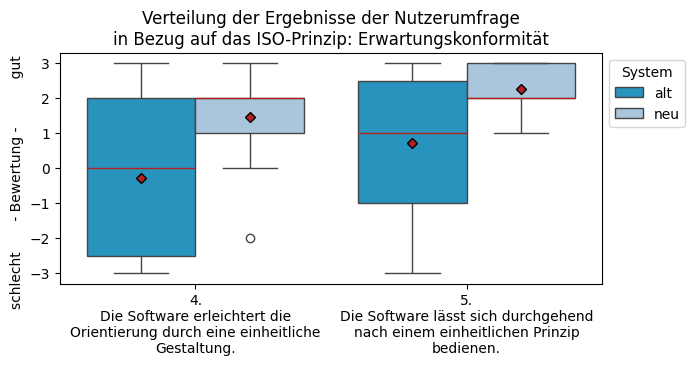
\includegraphics[width=1\linewidth]{Diagramme/pruemper_ek.png}
    \caption{Auswertung der Fragen bzgl. Gestaltungskriterium Erwartungskonformität nach ISO 9241-110 (Ausschnitt aus \autoref{fig:pruemper_all})}
    \label{fig:pruemper_Erwartungskonformität}
\end{figure}

\noindent
t-Test von Fragen 1 \& 8 sind signifikant (<0.5)\\
Boxplot: %\autoref{fig:pruemper_Erwartungskonformität}
